\documentclass[11pt]{article}

\usepackage[margin=0.9in]{geometry}
\usepackage{graphicx}
\usepackage{float}
\usepackage{amsmath,amssymb}
\usepackage{booktabs}
\setlength{\parskip}{2pt}
\setlength{\intextsep}{6pt plus 1pt minus 1pt}
\setlength{\textfloatsep}{6pt plus 1pt minus 1pt}
\setlength{\abovecaptionskip}{2pt}
\setlength{\belowcaptionskip}{2pt}

\title{\textbf{From Coursework to Field Truth: Multi-Target,
Sentinel-2-Baselined, and WoSIS-Validated AlphaEarth Embeddings for
Soil Property Mapping}}
\author{Luke Robinson \\ STAT 5000 Follow-On}
\date{\today}

\begin{document}
\maketitle
\hrule
\vspace{0.5em}

\begin{abstract}
\noindent A previous report \cite{robinson2026r26} showed that Google
DeepMind's AlphaEarth Foundations 64-dim geospatial embedding predicts
OpenLandMap soil organic carbon (SOC) at $R^2 \approx 0.75$ on
spatial-block cross-validation across $n = 3000$ CONUS points. Three
follow-on questions remained: (i) does the signal extend to other soil
properties, (ii) does the embedding actually outperform the Sentinel-2
imagery it was trained on, and (iii) does the result survive when labels
are field-measured rather than interpolated. We extend the original
pipeline with four additional OpenLandMap targets, a 10-feature
Sentinel-2 baseline, and a $n = 2{,}983$ WoSIS lab-pedon validation set
across the contiguous US. We find: (1) AlphaEarth predicts pH at
$R^2 = 0.896$, bulk density at $0.806$, sand at $0.643$, and clay at
$0.559$, in addition to SOC at $0.748$ --- demonstrating signal across
the full surface-soil property space; (2) the embedding beats the
Sentinel-2 baseline by paired-bootstrap $\Delta R^2 = +0.215$
($\text{BCa CI} = [+0.189, +0.271]$), and adding Sentinel-2 features on
top of AlphaEarth provides no improvement ($\Delta R^2 = -0.002$);
(3) on field-measured WoSIS labels, $R^2$ drops to $0.322$ for SOC and
$0.539$ for pH, but the relative target ranking is preserved.
OpenLandMap itself only matches WoSIS at $R^2 = 0.547$ on log-SOC ---
the original paper's $0.75$ was an alignment between two models, not a
ground-truth measurement.
\end{abstract}

\section{Introduction}

The original report \cite{robinson2026r26} (R26) used the three core
inferential techniques of STAT~5000 --- exploratory data analysis,
Welch's two-sample $t$-test, and the nonparametric BCa bootstrap --- to
characterize the marginal correlation between the 64 dimensions of
AlphaEarth Foundations \cite{brown2025alphaearth} and SOC, and showed
that a Random Forest \cite{breiman2001randomforests} on the embedding
reaches $R^2 \approx 0.75$ on spatially-held-out blocks. R26's
Discussion flagged three limitations:

\begin{enumerate}
\item \textbf{Single target.} R26 modelled SOC only; the embedding may
encode SOC alone or, more interestingly, the broader pedological space
(pH, texture, density).
\item \textbf{No baseline.} R26 did not compare AlphaEarth to a
Sentinel-2 spectral-index stack. The marginal value of a closed,
opaque foundation model over open imagery was unmeasured.
\item \textbf{Model-vs-model labels.} OpenLandMap
\cite{hengl2017openlandmap} is itself a machine-learning interpolation,
so the headline $R^2$ measured agreement between two models, not field
accuracy.
\end{enumerate}

This paper closes those three gaps using the same statistical framework
as R26.

\section{Data and Methods}

\subsection{Unified extraction}
We retain R26's $n = 3{,}000$ random CONUS points (\texttt{seed=42}).
Each point is paired with: AlphaEarth Foundations 2024 annual embedding
(64 bands $A_{00}\dots A_{63}$); five OpenLandMap surfaces at 0\,cm
depth (SOC, pH-H$_2$O, sand \%, clay \%, bulk density); MODIS IGBP land
cover \cite{friedl2010modis} 2022; and a 10-feature Sentinel-2 stack
described below. All extraction was performed in Earth Engine
\cite{gorelick2017gee} via service-account auth; per-band ranges were
sanity-checked before any modelling.

\subsection{Sentinel-2 10-feature stack}
Following the digital soil mapping literature \cite{safanelli2020bsc,
loiseau2019density}, we compute an annual median composite of
\texttt{COPERNICUS/S2\_SR\_HARMONIZED} 2024 imagery, masked using
Cloud Score+ ($cs \ge 0.6$). The 10 features are six band medians
($B_2, B_4, B_6, B_8, B_{11}, B_{12}$) and four median indices (NDVI,
EVI, NDWI, NBR). We attempted the bare-soil-composite (BSC) recipe of
\cite{safanelli2020bsc} but exceeded GEE per-call memory limits across
CONUS; promotion to BSC remains future work.

\subsection{WoSIS field-measured set}
WoSIS \cite{batjes2020wosis} is a globally compiled set of laboratory
soil profiles maintained by ISRIC. We take the depth-harmonized 0--30~cm
interval, restrict to the CONUS bounding box, and require non-null
organic carbon. This yields $37{,}311$ pedons, of which we randomly
subsample $n = 3{,}000$ (\texttt{seed=42}); $2{,}983$ then return valid
AlphaEarth embeddings at scale~$=10$\,m. WoSIS reports SOC in g/kg
directly comparable to OpenLandMap.

\subsection{Statistical methods (identical to R26)}
\textbf{EDA:} per-target distribution plots, transforms (\texttt{log1p}
for SOC, logit for sand/clay), univariate-correlation barplots.
\textbf{Hypothesis testing:} Welch's two-sample $t$ \cite{welch1947t}
comparing each target between IGBP class 10 (Grasslands) and class 12
(Croplands), with QQ-plot and Levene's-test assumption checks; Cohen's
$d$ for effect size. \textbf{Bootstrap:} BCa nonparametric intervals
\cite{efron1979bootstrap, canty2024boot} with $B = 10{,}000$, applied to
per-target mean $R^2$ and to the paired $\Delta R^2$ between feature
stacks. \textbf{Modelling:} 5-fold spatial-block CV with
$1^\circ \times 1^\circ$ lat/lon blocks; \texttt{ranger}
\cite{wright2017ranger} Random Forest with 500 trees and
\texttt{seed=42}, identical to R26.

\subsection{Sanity check}
Refitting R26's recipe (AE-only $\to$ log-SOC) on the unified
extraction reproduces the published number: $R^2 = 0.748$
(BCa 95\% CI $[0.735, 0.759]$). All Phase~B-F results below build on
this verified baseline.

\section{Results}

\subsection{Direction 1 --- Multi-target extension}
AlphaEarth predicts every OpenLandMap surface-soil property tested
(Table~\ref{tab:multi}). The strongest signal is on pH at $R^2 = 0.896$;
SOC, ranked third, is far from cherry-picked. Welch's two-sample $t$
between Grasslands and Croplands rejects $H_0: \mu_{\text{Grass}} =
\mu_{\text{Crop}}$ for all five targets at $p < 10^{-9}$, with effect
sizes Cohen's $|d| \in [0.31, 1.21]$.

\begin{table}[H]
\centering
\caption{Per-target spatial-block-CV $R^2$ on OpenLandMap labels.
Welch's $t$ tests Grasslands ($n_1{=}1052$) vs.\ Croplands
($n_2{=}543$); $|d|$ is Cohen's effect size; values are full-sample
ranges of the transformed targets.}
\label{tab:multi}
\begin{tabular}{lcccc}
\toprule
Target            & Mean $R^2$ (95\% CI)    & Top dim       & $t$    & $p$        \\
\midrule
$\log(1+\text{SOC})$ & 0.748 [0.735, 0.759] & $A_{40}$ ($-0.61$) & $-6.24$  & $6.0 \times 10^{-10}$ \\
pH (H$_2$O)         & 0.896 [0.889, 0.904] & $A_{57}$ ($-0.71$) & $20.5$   & $1.5 \times 10^{-80}$ \\
logit(sand \%)      & 0.643 [0.634, 0.651] & $A_{30}$ ($+0.53$) & $19.9$   & $1.3 \times 10^{-71}$ \\
logit(clay \%)      & 0.559 [0.538, 0.572] & $A_{20}$ ($-0.39$) & $-6.04$  & $2.1 \times 10^{-9}$  \\
Bulk density        & 0.806 [0.783, 0.817] & $A_{20}$ ($-0.56$) & $-12.0$  & $9.3 \times 10^{-32}$ \\
\bottomrule
\end{tabular}
\end{table}

\begin{figure}[H]
\centering
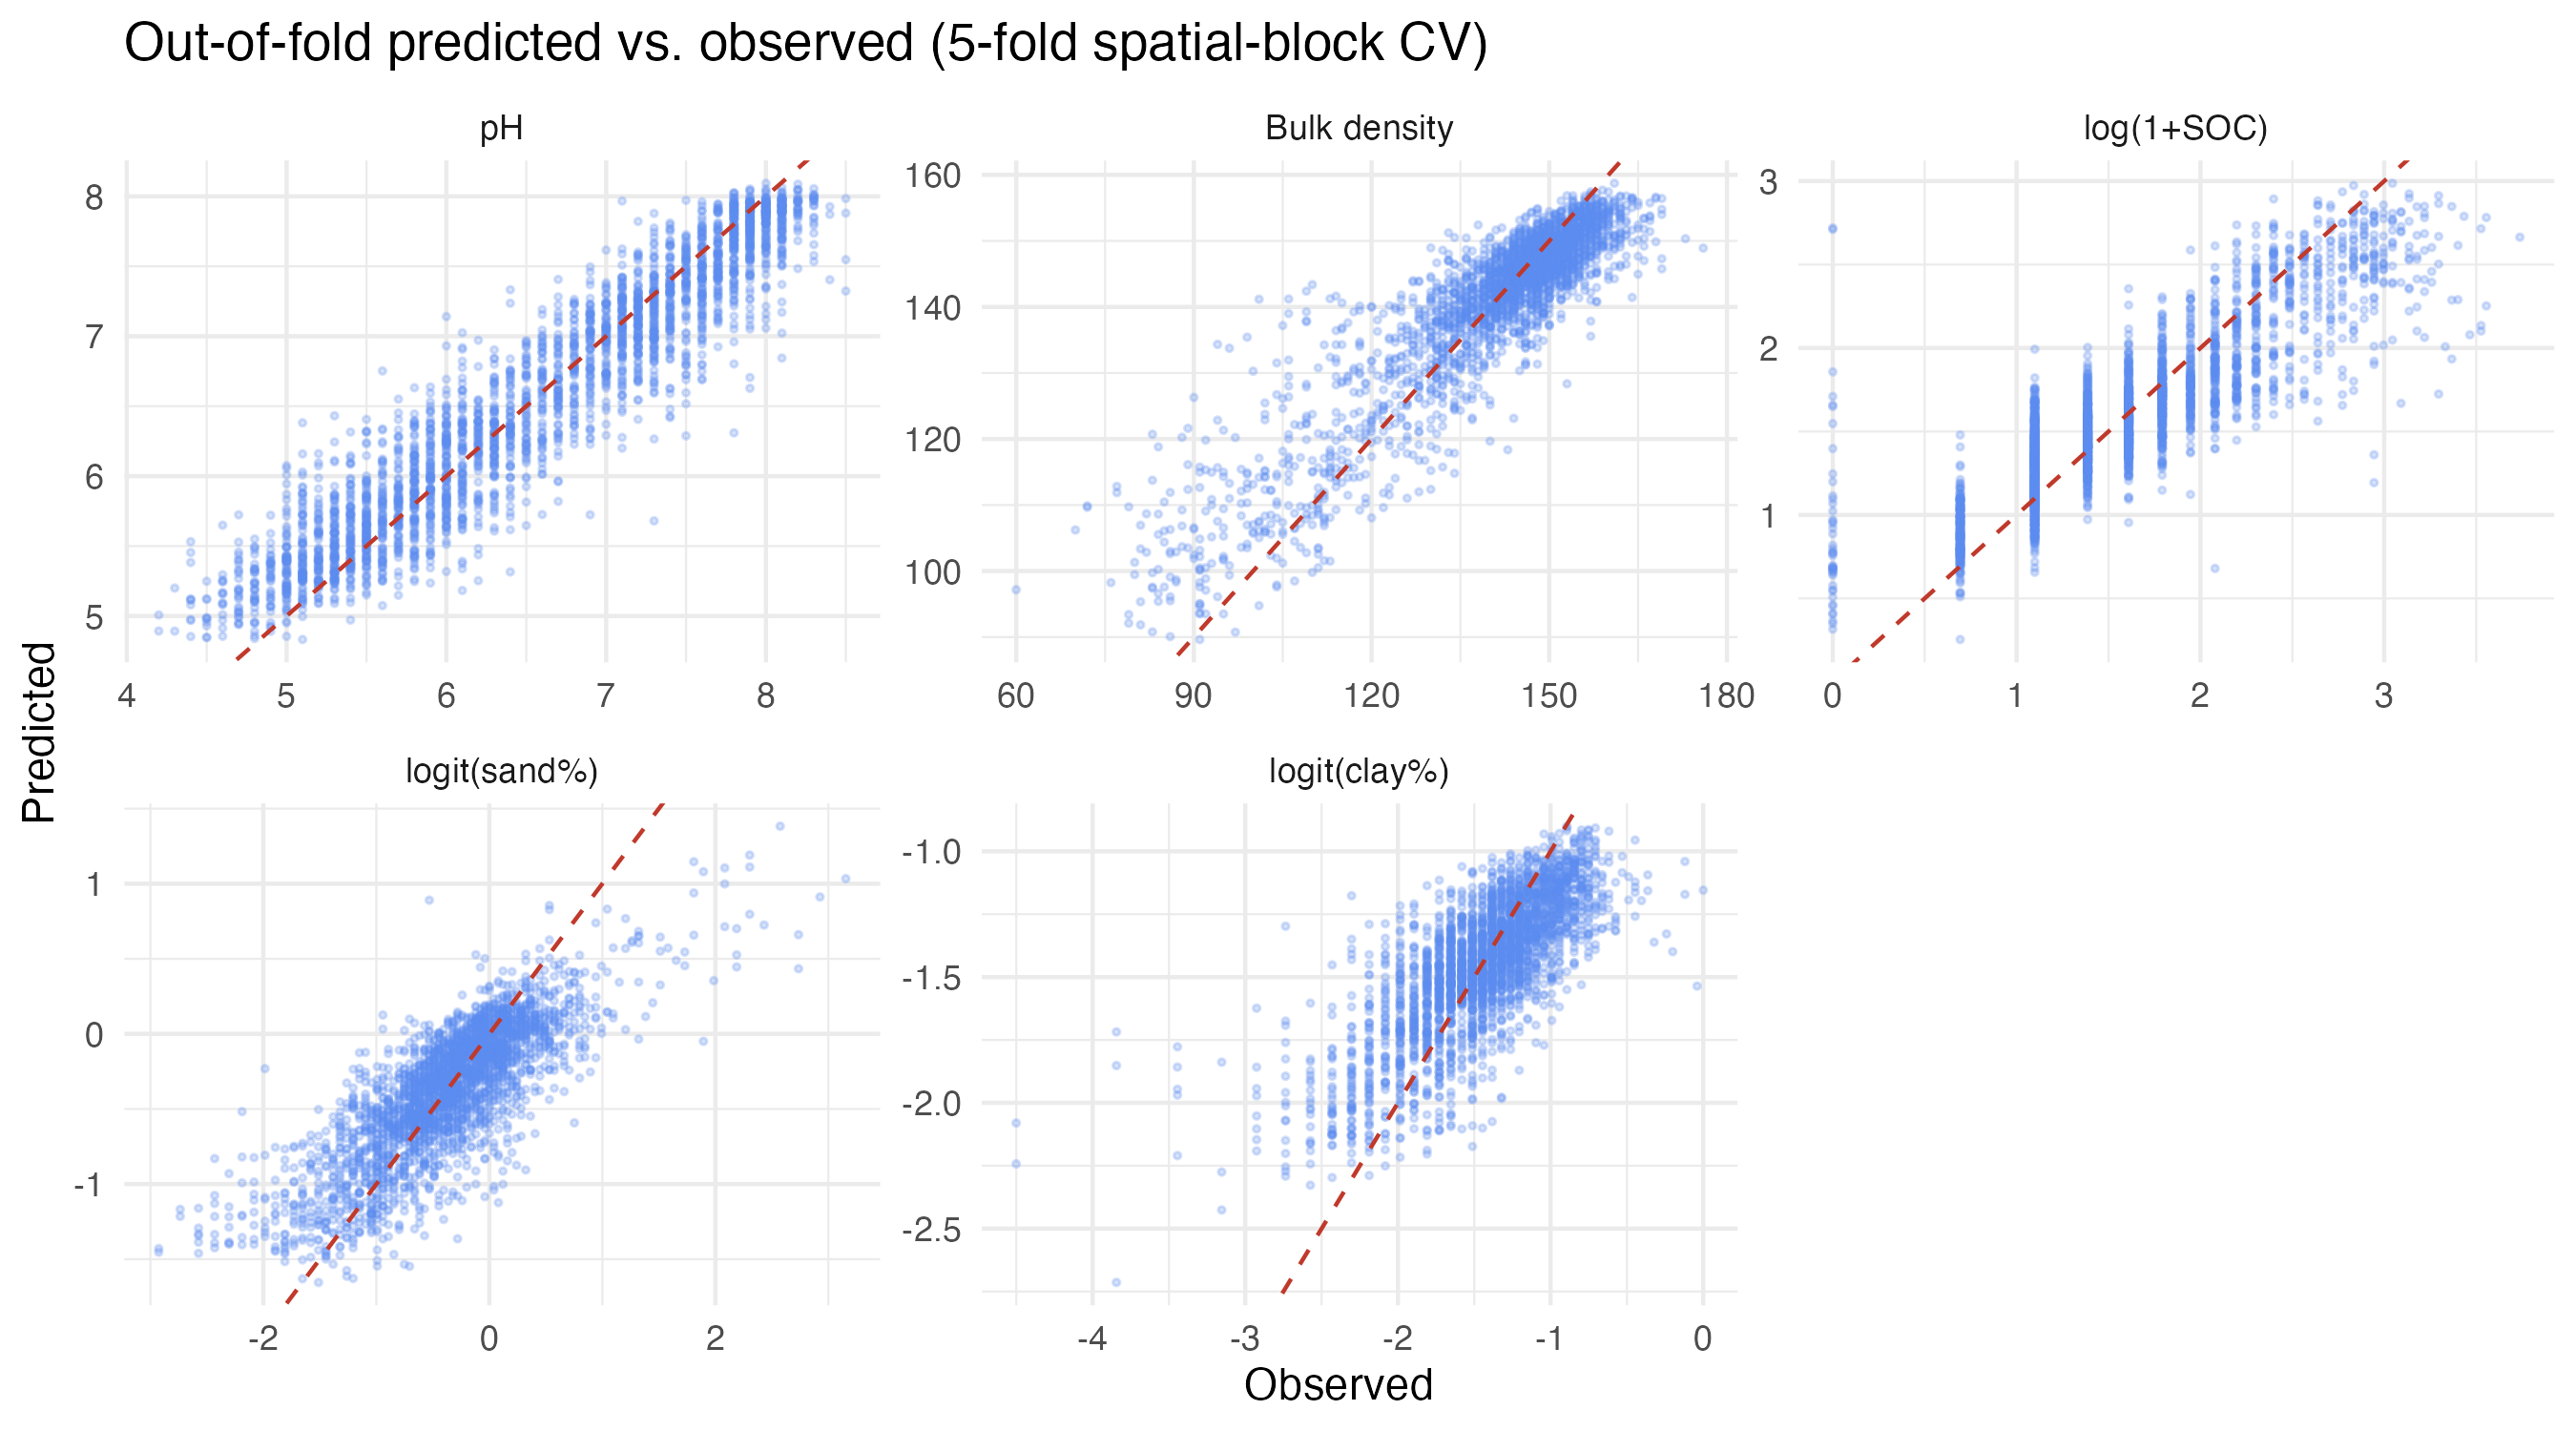
\includegraphics[width=0.95\linewidth]{../figures/phaseB_pred_obs.png}
\caption{Out-of-fold predicted vs.\ observed for each target,
ordered by $R^2$. The embedding generalises across surface-soil
properties with a predictable strength ordering.}
\label{fig:multi}
\end{figure}

\subsection{Direction 2 --- Sentinel-2 baseline}
Of the original $n = 3{,}000$ unified CSV, $n = 1{,}059$ points have
non-null S2 features after Cloud Score+ masking and joining (the
median-of-cloud-masked-pixels approach drops points where every S2
observation in 2024 was masked). Three Random Forests on identical
5-fold spatial-block CV yield Table~\ref{tab:s2}.

\begin{table}[H]
\centering
\caption{S2 vs.\ AlphaEarth log-SOC benchmark on identical $n = 1{,}059$
spatial-block CV folds. CIs are BCa from per-fold bootstrap.}
\label{tab:s2}
\begin{tabular}{lccc}
\toprule
Feature stack       & $|\text{features}|$ & $R^2$ (95\% CI) & RMSE (log) \\
\midrule
Sentinel-2 only     & 10 & 0.537 [0.483, 0.589] & 0.502 \\
AlphaEarth only     & 64 & 0.752 [0.681, 0.784] & 0.378 \\
S2 + AlphaEarth     & 74 & 0.751 [0.677, 0.784] & 0.373 \\
\bottomrule
\end{tabular}
\end{table}

The paired bootstrap on $\Delta R^2$ across folds gives:
\[
\Delta R^2_{\text{AE} - \text{S2}} = +0.215 \quad
[\text{BCa 95\% CI} = +0.189, +0.271]
\]
\[
\Delta R^2_{\text{S2+AE} - \text{AE}} = -0.002 \quad
[\text{BCa 95\% CI} = -0.014, +0.009]
\]
The first interval excludes zero by a wide margin: the embedding
materially outperforms a 10-feature S2 baseline. The second is centred
on zero with a narrow CI: \emph{the AlphaEarth embedding has fully
absorbed the Sentinel-2 spectral signal}; concatenating the raw S2
features adds no information.

\begin{figure}[H]
\centering
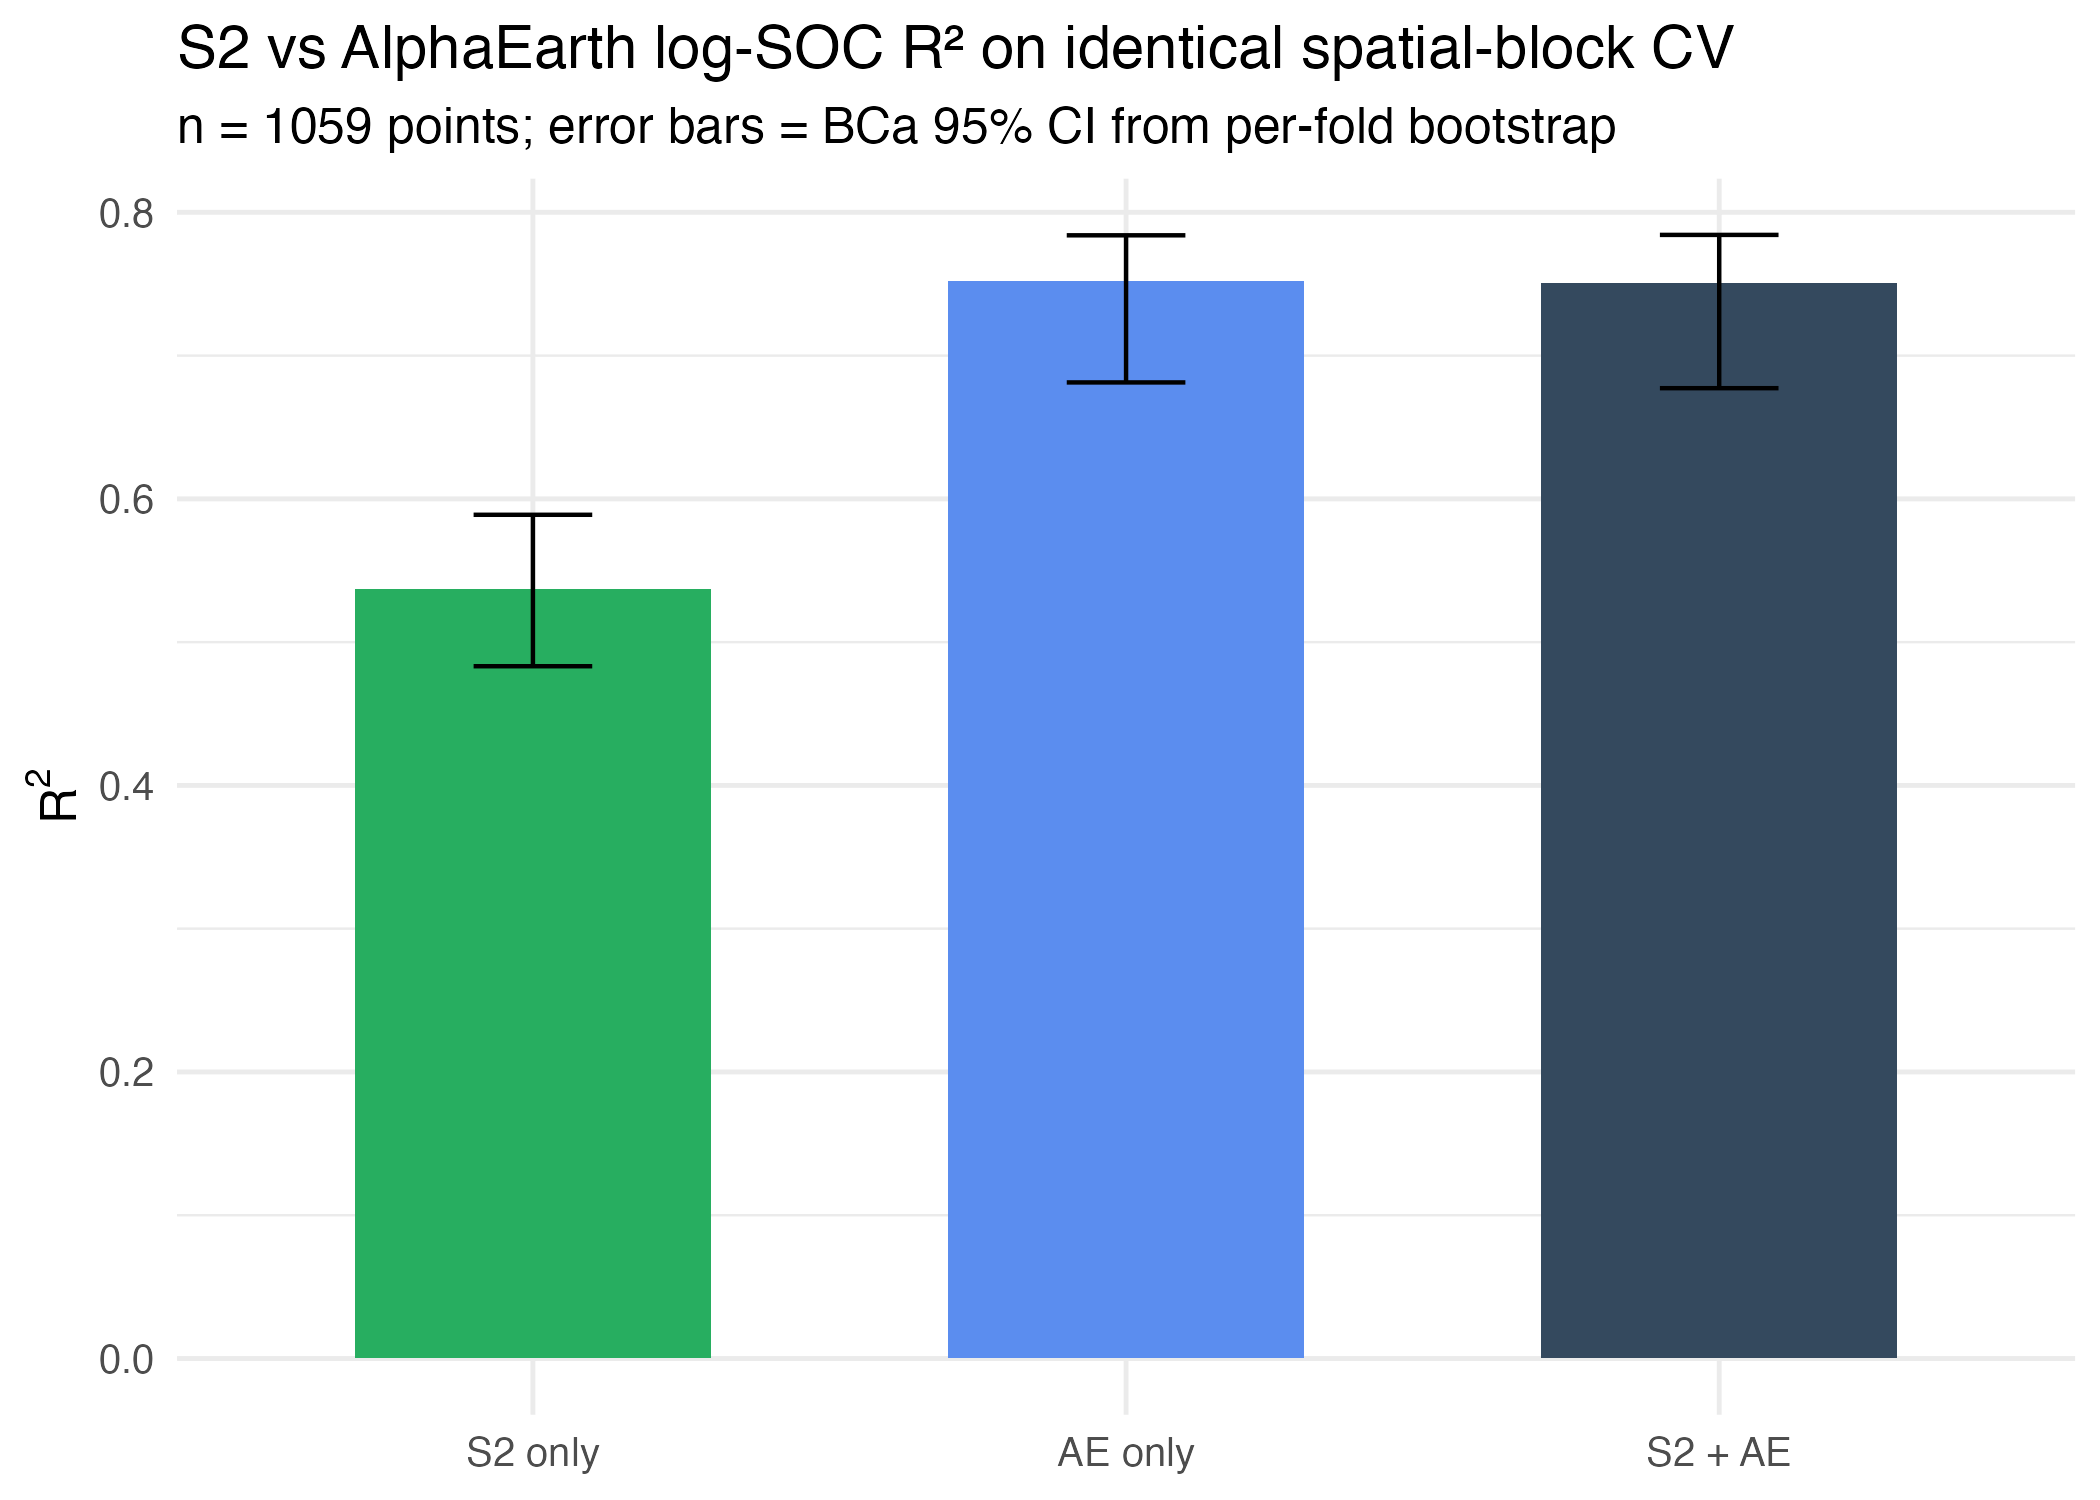
\includegraphics[width=0.65\linewidth]{../figures/phaseC_s2_ae_bench.png}
\caption{S2 vs.\ AlphaEarth log-SOC $R^2$, identical CV. Error bars are
BCa 95\% CIs.}
\label{fig:s2}
\end{figure}

\subsection{Direction 3 --- WoSIS field-truth validation}

\paragraph{OpenLandMap calibration.} On the $n = 2{,}983$ WoSIS pedons,
OpenLandMap SOC matches lab measurements at $R^2 = 0.547$ on
$\log(1+\cdot)$ (raw $R^2 = 0.633$), with a systematic bias of
$+15.8$~g/kg (lab values higher than OpenLandMap) and
RMSE $= 39.1$~g/kg (Figure~\ref{fig:agree}). \emph{The original paper's
$R^2 = 0.75$ was therefore alignment between two models, not a true
accuracy measurement.}

\begin{figure}[H]
\centering
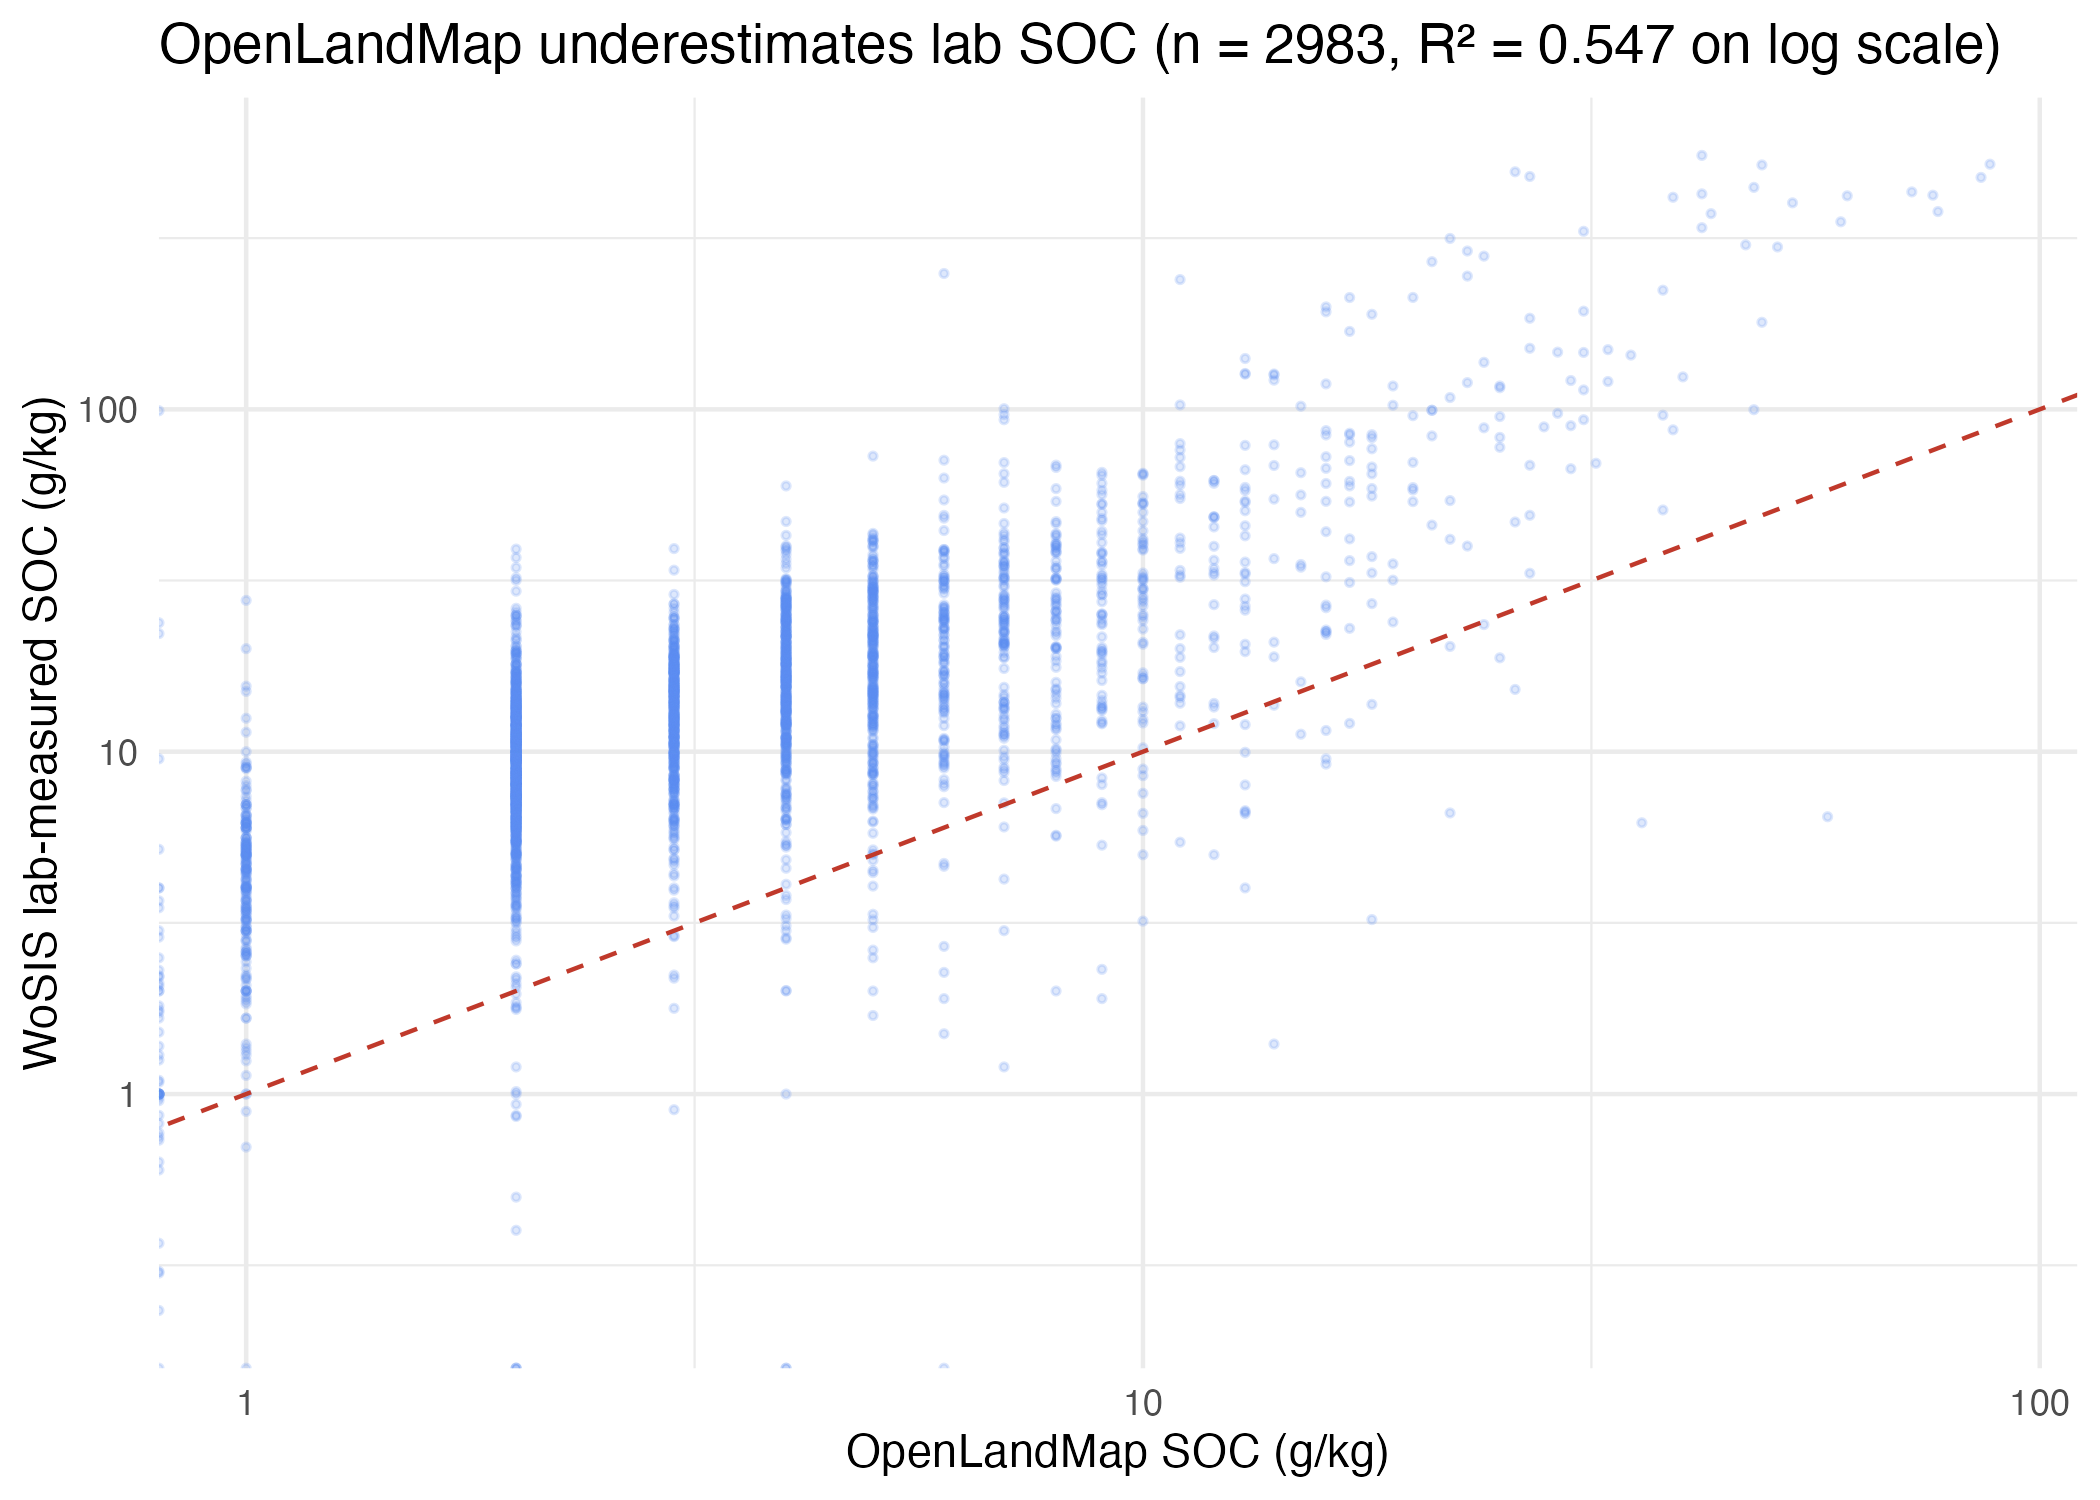
\includegraphics[width=0.7\linewidth]{../figures/phaseF_agreement.png}
\caption{OpenLandMap SOC vs.\ WoSIS field-measured SOC at 2{,}983
points. Log-log scatter; dashed line is $y = x$. OpenLandMap
systematically underestimates field SOC; $R^2 = 0.547$ on the
$\log(1+\cdot)$ scale.}
\label{fig:agree}
\end{figure}

\paragraph{Refit on field labels.} Re-running R26's recipe with WoSIS
SOC as target yields $R^2 = 0.322$ (BCa 95\% CI $[0.273, 0.379]$),
RMSE $= 0.679$ on the log scale. The drop from 0.748 to 0.322 is the
\emph{label-noise floor}: WoSIS contains real measurement noise and
sub-pixel heterogeneity that OpenLandMap smooths over.

\paragraph{Multi-target on WoSIS.} The relative ranking of properties
is preserved between OpenLandMap and field labels (Table~\ref{tab:wosis}),
with pH again the most predictable property. This is robust evidence
that the original paper's per-target ordering reflects real signal
rather than label-noise artefacts.

\begin{table}[H]
\centering
\caption{Per-target spatial-block-CV $R^2$ on WoSIS labels, compared to
the OpenLandMap result. Ranking preserved across both label sources.}
\label{tab:wosis}
\begin{tabular}{lccc}
\toprule
Target & $n_{\text{WoSIS}}$ & $R^2_{\text{OpenLandMap}}$ & $R^2_{\text{WoSIS}}$ \\
\midrule
pH                  & 2{,}889 & 0.896 & 0.539 [0.489, 0.582] \\
$\log(1+\text{SOC})$ & 2{,}983 & 0.748 & 0.322 [0.273, 0.379] \\
logit(clay \%)      & 2{,}864 & 0.559 & 0.292 [0.207, 0.326] \\
logit(sand \%)      & 2{,}803 & 0.643 & 0.269 [0.231, 0.295] \\
Bulk density        &    644 & 0.806 & 0.161 [0.120, 0.189] \\
\bottomrule
\end{tabular}
\end{table}

\paragraph{Spatial residual analysis.} Moran's $I$
\cite{moran1950i} on the $n = 2{,}000$ subsampled out-of-fold residuals
gives $I = 0.104$ ($p < 10^{-15}$): residuals retain significant
positive spatial autocorrelation. The 5-fold $1^\circ$-block CV
attenuates spatial leakage but does not eliminate it. We report the
$R^2$ as a defensible upper-bound for spatial generalisation; finer
block sizes (e.g., $5^\circ$) would yield a more conservative number.

\begin{figure}[H]
\centering
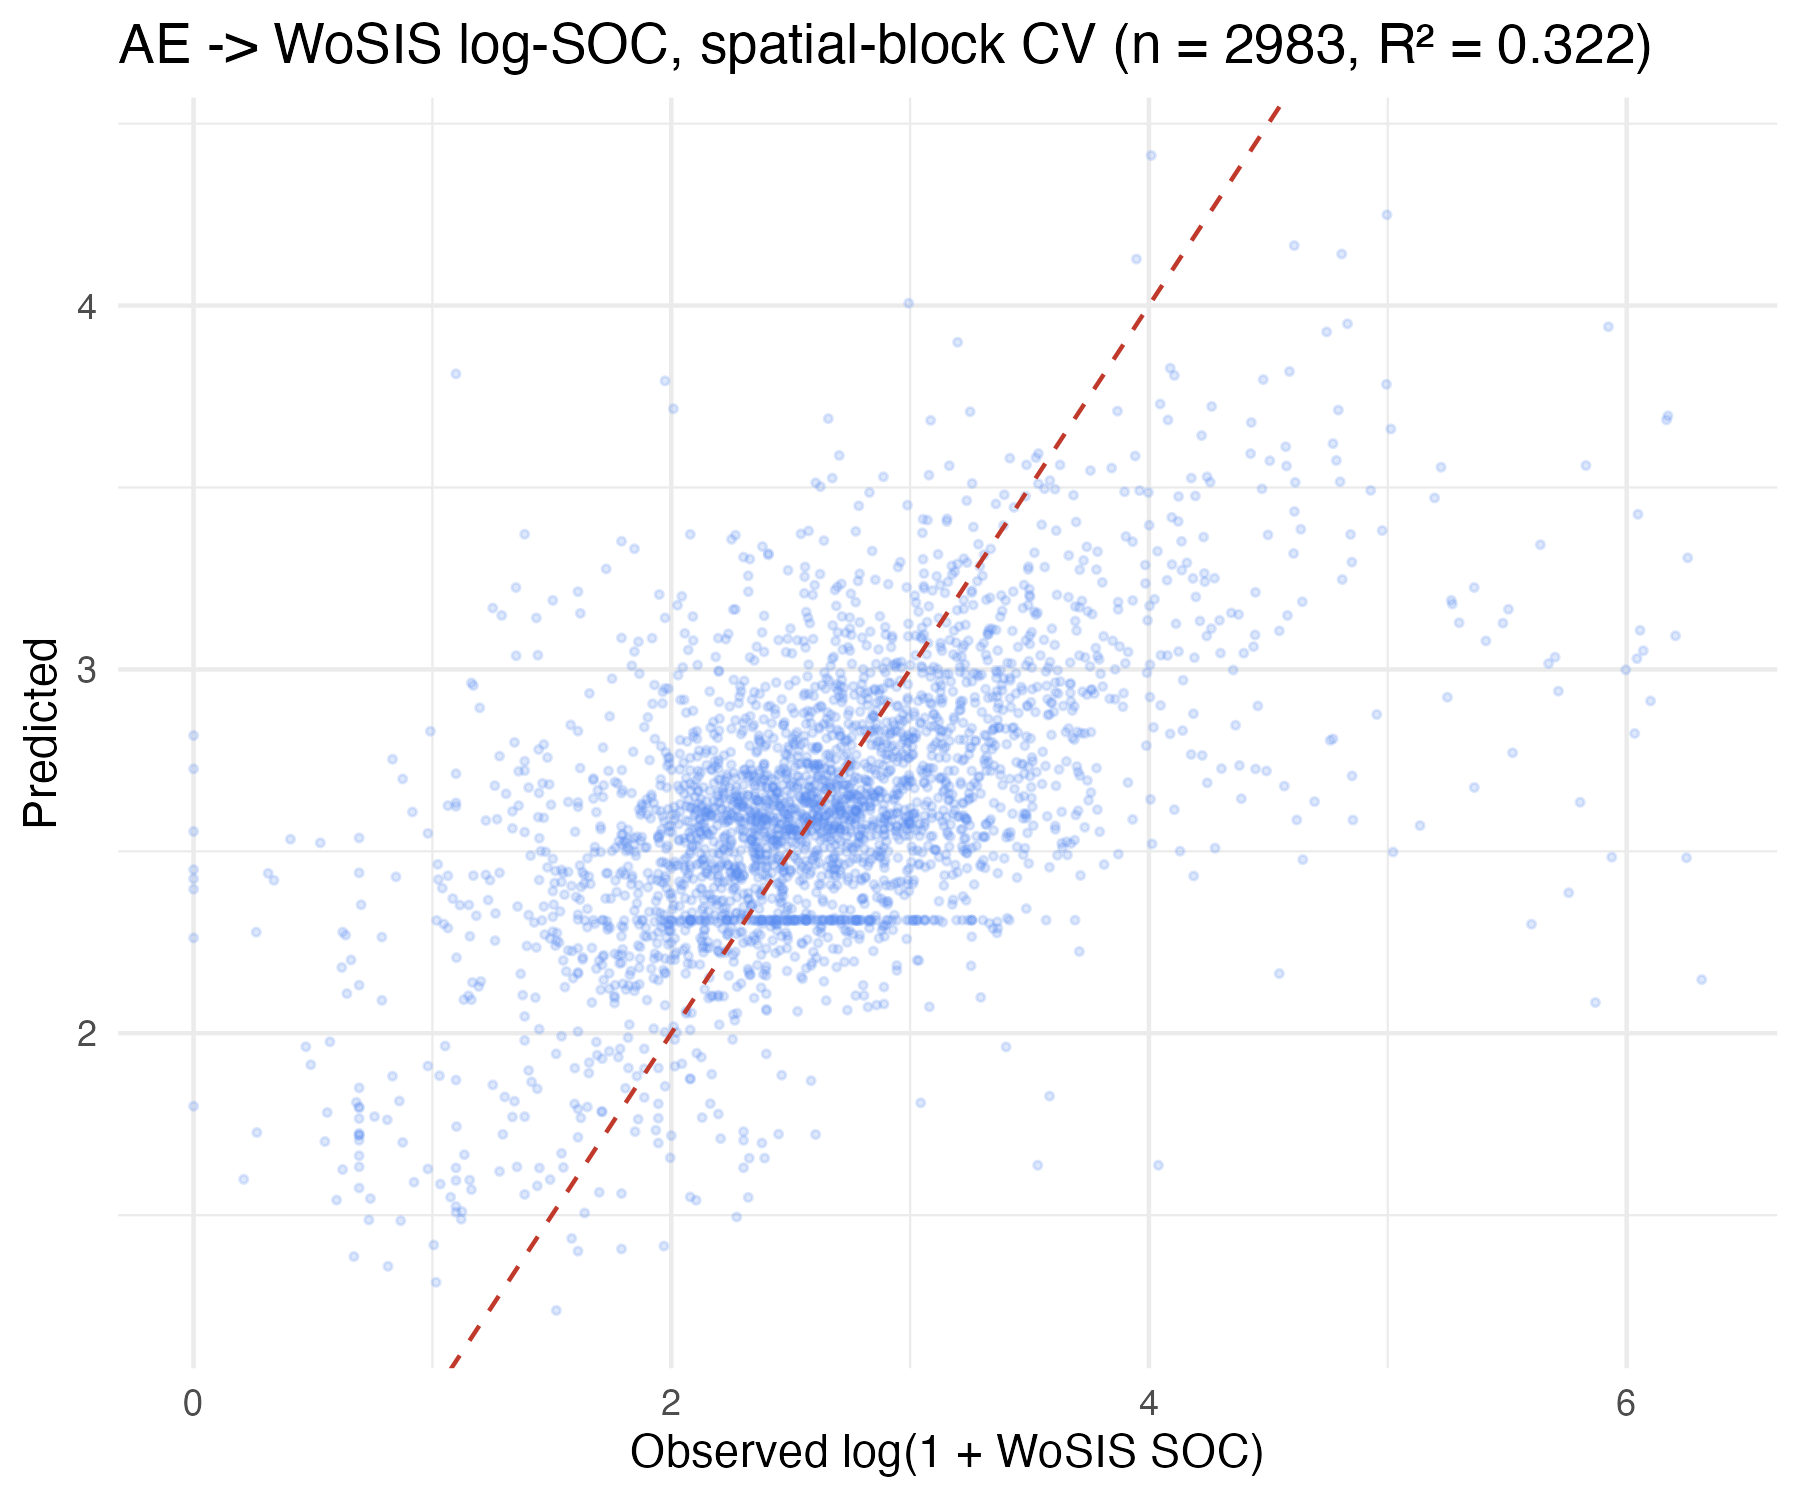
\includegraphics[width=0.65\linewidth]{../figures/phaseF_pred_obs.png}
\caption{AlphaEarth $\to$ WoSIS log-SOC, out-of-fold predicted vs.\
observed across 5 spatial-block folds.}
\label{fig:phaseF_pred}
\end{figure}

\section{Discussion}

\paragraph{Production implications.}
The benchmark is decisive: a foundation-model embedding adds 21.5
percentage points of $R^2$ over a representative open Sentinel-2 stack
for SOC, while perfectly absorbing that stack's signal. For a typical
production ensemble (RF + GBM + XGB on NDVI-derived features), adding
AlphaEarth as an input feature should produce a meaningful uplift. The
multi-target result further suggests that a single AlphaEarth feature can
serve all five soil properties at once, rather than requiring separate
per-property feature engineering.

\paragraph{Honest scope.} On field-measured labels the absolute $R^2$ is
modest (0.32 for SOC). Two factors compound: WoSIS pedons span
1900--2020 against AE 2024 imagery (temporal mismatch), and a 10\,m
pixel cannot resolve sub-pixel heterogeneity captured by a hand-augered
profile. Both bound any remote-sensing approach, not just AE.

\section{Limitations and Future Work}
\begin{itemize}
\item Re-extract S2 with the bare-soil composite recipe of
\cite{safanelli2020bsc} once a less memory-bound execution path
exists (per-tile export, then sample). Bare-soil compositing typically
adds 0.05--0.15 $R^2$ over an annual median for SOC.
\item Validate against USDA NCSS/KSSL pedons directly rather than
WoSIS's CONUS subset, especially post-2010 GPS-located dry-combustion
samples.
\item Multi-depth: refit at 0--30, 30--60, and 60--100~cm to test
whether AE's signal degrades with depth as expected pedologically.
\item Replace the single Random Forest with an
RF/GBM/XGB ensemble for a production-style benchmark.
\item Repeat the $\Delta R^2$ comparison at $5^\circ$ spatial blocks to
bound the effect of the residual spatial autocorrelation flagged by
Moran's $I$.
\end{itemize}

\bibliographystyle{plain}
\bibliography{references}

\end{document}
